% !TeX program = xelatex
\documentclass[11pt, a4paper, UTF8, fontset=fandol]{ctexart}

\usepackage{amsmath, amssymb}
\usepackage{booktabs, multirow, array, longtable}
\usepackage{threeparttable}
\usepackage{graphicx}
\usepackage{geometry}
\usepackage{tikz}
\usetikzlibrary{positioning, arrows.meta, shapes.geometric, calc, fit, backgrounds, decorations.pathmorphing, shadows}
\usepackage{hyperref}
\usepackage{float}
\usepackage{algorithm}
\usepackage{algorithmic}
\renewcommand{\algorithmicrequire}{\textbf{输入:}}
\renewcommand{\algorithmicensure}{\textbf{输出:}}
\geometry{left=2.3cm, right=2.3cm, top=2.5cm, bottom=2.5cm}
\hypersetup{colorlinks=true, linkcolor=black, citecolor=black, urlcolor=blue}

% 兼容部分 pdflatex 环境中 CJK 粗体字体缺失问题
\makeatletter
\renewcommand{\bfdefault}{m}
\makeatother

\ctexset{ section={format=\Large\rmfamily}, subsection={format=\large\rmfamily}, subsubsection={format=\normalsize\rmfamily} }

\begin{document}
    % 手工标题区：避免 \maketitle 默认粗体中文触发字体缺失
    \begin{center}
        {\Large Trust Flow-Driven Trusted Federated Learning in Edge Computing: A Study on Key Technologies\par}
        \vspace{4pt}
        {\Large 边缘计算中信任流驱动的可信联邦关键技术研究\par}
        \vspace{10pt}
        {周家凯\par}
        \vspace{2pt}
        {2026年3月\par}
    \end{center}

    \begin{abstract}
        近年来，联邦学习以其数据不出本地仅交换参数的范式促进隐私保护下的多方模型协同优化，已成为边缘智能的关键支撑。然而，在愈加开放的边缘计算场景中，非独立同分布（Non-IID）数据、终端设备异构化、不可信客户端等情形叠加，导致现有的鲁棒聚合方法面临着严峻挑战。由此，本文从软硬件协同角度提出一种基于全流程信任流的可信联邦聚合机制。首先，该机制融合基于可信执行环境（TEE）的远程证明和运行监测方法，以从本地模型训练阶段就约束参与客户端的强制准入与执行完整性验证；其次，通过刻画客户端的长期历史贡献和短期行为风险，设计了基于客户端信任状态的双流正交信誉演化方法，以分解客户端信任状态为历史效用流和瞬时风险流，解决潜伏攻击的跨轮识别挑战；最后，提出了基于纯净参考方向的分层差异化聚合方法，融合按层门控、重归一化和动态裁剪思想，以在聚合阶段抑制恶意更新并保留合法异构贡献，缓解 Non-IID 下泛化能力下降问题。基于 Flower 平台在 CIFAR-10 数据集上的 20 客户端、6 类混合攻击实验结果表明，本文机制在保证模型精度达到 $92.31\% (\pm 0.09\%)$ 的同时，将后门攻击成功率（ASR）控制在 $10.21\% (\pm 0.05\%)$，且正常客户端的永久误杀率趋近于 0。
    \end{abstract}

    关键词：联邦学习；边缘计算；可信执行环境；风险状态建模；分层鲁棒聚合；后门防御

    \begin{center}
        Abstract
    \end{center}
    In recent years, federated learning has become a key enabler of edge
    intelligence by supporting collaborative model optimization under privacy
    constraints through the paradigm of keeping data local and exchanging only
    model parameters. However, in open edge-computing environments, the combined
    effects of non-independent and identically distributed (Non-IID) data,
    device heterogeneity, and untrusted clients expose significant tradeoffs
    among security, robustness, and generalization for existing robust
    aggregation methods. To address this issue, we propose a trust-flow-driven
    trusted federated aggregation mechanism that covers client admission, runtime
    monitoring, and secure aggregation from a hardware-software co-design
    perspective. First, remote attestation and runtime monitoring based on
    trusted execution environments (TEEs) are integrated to enforce client
    admission and verify execution integrity during local training. Second, to
    identify stealthy attacks across training rounds, we design an orthogonal
    dual-stream reputation evolution method centered on client trust states,
    decomposing them into a historical utility stream for long-term contribution
    and an instant risk stream for short-term anomalous behavior, thereby
    providing persistent dynamic trust signals for subsequent auditing and
    aggregation control. Third, we propose a layer-wise
    differentiated aggregation strategy guided by a clean reference direction.
    By combining layer-wise gating, weight re-normalization, and dynamic
    clipping, the method suppresses malicious updates while preserving legitimate
    heterogeneous contributions, thereby mitigating the degradation of
    generalization under Non-IID settings. Experiments on Flower with CIFAR-10
    under 20 clients and six mixed attack types show that the proposed mechanism
    achieves an average accuracy of 92.31\% ($\pm$ 0.09\%) while limiting the
    attack success rate (ASR) to 10.21\% ($\pm$ 0.05\%), with the permanent false
    positive rate on benign clients approaching zero.

\section{引言}
当前，随着终端设备所具备的计算能力愈加强大，越来越多的终端设备能够高效地利用本地数据支持本地模型训练，同时，为更好地以聚合多终端训练经验以支持多方模型协同优化并保护各设备的本地数据隐私，联邦学习范型被深入研究\cite{kairouz2021flsurvey}，其所具备的数据不出本地仅通过模型参数交换的特性被广泛应用于模型的分布式协同训练场景，已然成为边缘智能发展的关键支撑技术。然而，随着万物互联构成的网络环境愈加开放，基于联邦学习的经验聚合以促进模型协同优化所面临的性能瓶颈不再局限于模型结构和优化器设计层面，聚合阶段的可信性和稳健性日益成为影响整体可用性的关键因素。因为在实际应用场景中，不仅各边缘设备端的数据分布具有异构性且处理能力也有显著差异，另外，模型协同优化的各参与方相关行为也难以完全约束，这些特征在经验聚合时显然会放大统计偏移和带来安全风险。

在通常的联邦学习范型中，客户端完成本地数据处理及本地模型训练后，会将模型相关参数上传，服务端聚合各客户端模型参数后会下发更新后的模型参数，以此通过多轮迭代直至收敛，显然，上述流程在实际愈加开放的万物互联多边缘网络环境下面面临着多重风险。具体来说，首先，开放的训练环境缺少强制完整性约束，恶意客户端可以绕过真实训练而直接构造并上传模型参数，也会极大地影响服务端对聚合参数真实性的判断能力，一些研究工作提出了基于可信执行或可验证训练的方法\cite{lu2025tmt,zhang2025rppfl,r1_tee_integrity}，以硬件远程证明等方式保证客户端对模型训练的真实性，但仍然缺乏应对训练过程真实而模型更新却嵌入恶意特征等手段。其次，恶意客户端实施参数投毒、隐蔽后门等攻击\cite{gu2017badnets,wang2019neuralcleanse}，通过将恶意触发特征嵌入常规更新分布参数中，会显著降低单轮检测成功率，一些研究工作提出了基于时序信誉与相似性的方法\cite{cao2021fltrust,fung2020foolsgold}，通过引入跨轮信息来缓解单轮判断的不稳定问题，但对于恶意客户端前期积累信誉后期持续小幅度投毒等潜伏式攻击显然存在识别滞后问题，而且，单一信誉分与固定阈值机制对深层异常触发特征的识别能力也有很大不足。

另外，不同设备的非独立同分布数据（Non-IID）会增加最优更新的方向离散度，很容易模糊正常波动和异常偏移之间的边界，导致强 Non-IID 条件下鲁棒性和泛化性之间的冲突，一些研究工作提出了基于距离排斥或统计截断等的方法抑制异常更新\cite{blanchard2017krum,yin2018byzantine}，还有一些研究工作通过自适应权重调整来缓解异构影响\cite{wang2025rasa}，但强长尾分布情形下，这些方法会将合法偏移的参数更新误判为异常参数，可能导致关键异构信息被过度剔除而显著降低模型泛化能力。在实际场景中，上述执行环境更加开放、跨轮潜伏攻击、强异构统计偏移等挑战往往不会单独出现，尤其是在万物互联的边缘智能场景中数个因素很可能出现叠加出现的情形，很容易导致诸如拦截阈值收紧误杀率上升、拦截阈值放宽漏检率增加等多种难以权衡的难题。由此，如何构建覆盖全流程的统一状态建模与联动决策机制，在兼顾客户端本地模型训练的准入及可信和聚合时对客户端低误杀率且高召回率的要求下，维持模型协同优化的收敛和泛化性能成为亟需解决的关键问题。

为应对以上所述的三个主要难题，本文从软硬件协同角度提出一种基于全流程信任流的可信联邦聚合机制。在该机制中，我们首先引入了面向客户端模型训练的远程证明及其运行监测方法，利用 TEE 环境内部熵变分析和卡尔曼滤波，从各终端设备的客户端侧建立强制准入与执行时的可信能力，解决了传统环境执行完整性缺失的问题，为硬件证明与软件风险评估的时序联动提供关键支撑；然后，我们设计了基于客户端信任状态的双流正交信誉演化方法，从客户端的长期历史贡献和短期行为风险相结合的角度评估各参与方的信任状态，其中引入贝叶斯推断（Beta信誉系统）建模长期历史效用，并结合瞬时风险流构建融合长期积累和瞬时熔断的联合机制，有效增强了对于潜伏攻击的跨轮识别能力；最后，我们提出了基于纯净参考方向的分层差异化聚合方法，在聚合阶段融合了按层门控、重归一化和动态裁剪的思想，以此应对强长尾分布带来的泛化性冲突，在抑制多模型聚合时存在的恶意更新同时保留合法异构的贡献，进而缓解 Non-IID 下整体泛化能力下降问题。

本文的主要贡献总结如下：
\begin{enumerate}
    \item \textbf{提出软硬件协同的信任流防御框架}。通过“TEE 准入验证 + 运行监测 + 内容审查 + 状态演化 + 分层聚合”构建覆盖“准入-监测-聚合”的全流程闭环防线，覆盖从客户端接入到模型更新的完整路径。
    \item \textbf{提出贯穿全过程的双流正交信誉演化机制}。将客户端状态拆分为历史效用流（HistPerf）与瞬时风险流（RiskEMA），分别处理长期贡献与短时异常，并作为后续审查、状态转移与聚合控制的核心依据，在设定条件下兼顾高恶意召回与低永久误杀。
    \item \textbf{设计基于纯净参考的分层差异化聚合策略}。利用服务器侧参考方向与按层风险门控，实现逐层准入、幸存者重归一化与动态 L2 裁剪，降低深层后门透传风险。
    \item \textbf{完成端到端实现与实证验证}。在 Flower 平台完成 20 客户端、6 类混合攻击实验（$n=5$）；结果显示框架在高对抗设置下仍保持 $92.31\% (\pm 0.09\%)$ 精度、$10.21\% (\pm 0.05\%)$ ASR，以及接近 0 的永久误杀率。
\end{enumerate}


\section{背景与相关工作}

\subsection{联邦学习与边缘计算协同架构}
联邦学习（Federated Learning, FL）在“数据不出本地”的约束下，通过参数协同完成全局模型训练。在边缘计算场景中，端-边-云（Client-Edge-Cloud）的架构模式已被广泛采用：边缘侧负责本地训练并上传更新，中心服务器负责聚合与模型下发。

在标准的 FL 设置中，全局优化目标为最小化所有客户端数据分布上的经验风险：
\begin{equation}
\min_{W} \mathcal{L}(W) = \sum_{k=1}^K p_k \mathcal{L}_k(W)
\end{equation}
其中 $p_k = |\mathcal{D}_k| / \sum |\mathcal{D}_j|$ 为数据量占比。在第 $t$ 轮，服务器下发全局模型 $W_{global}^{(t-1)}$，客户端 $k$ 以其为初值在本地数据上执行 $E$ 轮学习率为 $\eta_l$ 的 SGD，得到本地更新：
\begin{equation}
\Delta W_{k}^{(t)} = W_{k, E}^{(t)} - W_{global}^{(t-1)}, \quad \text{其中 } W_{k, e}^{(t)} = W_{k, e-1}^{(t)} - \eta_l \nabla \mathbb{E}[\ell(W_{k, e-1}^{(t)}; x, y)]
\end{equation}
其中，期望 $\mathbb{E}[\cdot]$ 表示对本地数据集 $\mathcal{D}_k$ 的 mini-batch 采样期望。随后，客户端上传更新量，服务器执行某种形式的参数聚合：$W_{global}^{(t)} = W_{global}^{(t-1)} + \mathrm{Agg}(\{ \Delta W_{k}^{(t)} \}_{k\in\Phi})$。

但是该架构天然存在通信延迟、设备异构和数据 Non-IID 等问题。为缓解这些挑战，已有研究提出簇式联邦（Clustered FL）\cite{r9_clustered}、自适应剪枝扩展（FedPE）\cite{fedpe} 和拆分式联邦（ParallelSFL）\cite{parallelsfl} 等方法。但随着系统复杂度提升，攻击面也随之扩大，恶意节点也更易潜伏并影响训练过程。

\subsection{边缘伪装、模型投毒与隐蔽后门攻击}
在开放且缺少强制准入的联邦网络中，服务器难以准确判断客户端身份与更新质量，攻击手段主要分为两类：其一是\textbf{无目标投毒}（Untargeted Poisoning），如 Sign-flipping 与 Gradient Scaling，目标是破坏全局收敛并造成拒绝服务；其二是\textbf{目标后门攻击}（Targeted Backdoor），如标签翻转、干净标签污染和语义后门，通过隐蔽触发器在推理阶段诱导定向误分类。

\subsection{现有主动防御防线的机制与不可调和的局限性}
为应对上述威胁，早期防御多依赖几何统计过滤，例如 Krum\cite{blanchard2017krum} 与 Trimmed Mean\cite{yin2018byzantine}。近期的研究进一步引入了时序信任评估，如 FLTrust\cite{cao2021fltrust}、FoolsGold\cite{fung2020foolsgold} 与 RaSA\cite{wang2025rasa}，并在恶意检测\cite{dou2025toward}、可信训练框架\cite{lu2025tmt}、分级保护\cite{wang2024federated} 等方向持续扩展。针对后门与合谋攻击，也已有 FLPurifier\cite{flpurifier}、RoseAgg\cite{roseagg} 和 ShieldFL\cite{shieldfl} 等方案。
但纯软件防御在强 Non-IID 与高权限攻击下仍有明显短板：阈值收紧会抬高误杀率（FPR），阈值放宽又可能放过潜伏攻击；同时，当攻击者控制底层环境时，缺少硬件信任根的软件探针难以形成完整闭环。

\subsection{联邦环境下的可信硬件信任根 (TEE)}
为补齐物理可信的缺口，研究开始引入 Intel SGX、ARM TrustZone 等可信执行环境（TEE）。TEE 通过隔离执行与受保护内存保证关键代码和密钥材料的完整性，即便宿主操作系统被攻陷，攻击者也难以直接篡改证明流程\cite{liao2024verifiable,zhang2025rppfl}。现有的工作表明，TEE 在训练完整性\cite{r1_tee_integrity}、威胁缓解\cite{r5_tee_mitigating} 和工业 IoT 信任共享\cite{r12_iot_tee} 中具备现实价值，其在 SGX 环境下的联邦扩展与效率优化也得到验证\cite{xu2021distributed,yan2024efficient}。
本文在此基础上构建软硬件协同防御体系。与仅做静态加密或单维异常评测的方法不同，本文将硬件远程证明（Remote Attestation）与双流信誉演化进行时序耦合：云端负责参数审查，边缘侧 TMAA 提供可信证据与运行时监测，实现“强制准入 + 动态熔断”的联动防护。


\section{系统模型与问题定义}

\subsection{端边云协同架构与系统流转建模}
本文考虑一个典型的端-边-云（Client-Edge-Cloud）异构通信环境（见图~\ref{fig:system_arch}）。系统由中心\textbf{聚合服务器（Server, $\mathcal{S}$）}与 $K$ 个边缘客户端组成，记为 $\mathcal{C}=\{c_1, c_2, \dots, c_K\}$。客户端可能动态上下线，且部分节点可能被攻击者控制。

\begin{figure}[htbp!]
    \centering
    
\includegraphics[width=0.90\textwidth]{system_arch.pdf}
    \caption{联邦计算网络交互：基于 TEE 锚点加密的端边云协同物理架构图}
    \label{fig:system_arch}
\end{figure}

基于上述网络交互拓扑，本文提出的信任流驱动可信联邦框架在端云之间构建了一条完整的信任传递与评估链路。系统的整体工作流程与主要物理实体模块的相互关系定义如下：

\begin{enumerate}
    \item \textbf{边缘客户端侧（可信执行与特征提取）}：每个接入的客户端需配备可信执行环境（TEE）及部署其内的可信管理代理（TMAA）。在本地训练阶段，TMAA 不仅负责在训练前生成远程证明报告（Attestation Quote）以静态验证执行环境的完整性，还会持续监测训练过程中的关键行为特征序列（如梯度方向变化、损失值波动等）。随后，利用信息熵和卡尔曼滤波进行初步的动态信任评估，连同模型更新参数一并上传至云端。
    
    \item \textbf{中心服务器侧（审查、演化与聚合控制）}：服务器作为全局协调者，接收到客户端的更新及信任证明后，执行基于信任流的三阶联动防御。首先进行\textbf{内容审查}，提取纯净参考方向并利用余弦相似度计算高维更新质量；其次进入\textbf{双流状态演化}，利用 Beta 贝叶斯推断建立历史效用流以评估长期贡献，并结合多维最大值探针更新瞬时风险流以识别突发异常；最后执行\textbf{分层鲁棒聚合}，根据不同网络层的安全敏感度进行差异化门控裁剪与幸存者权重重归一化，得到全局安全更新并下发。
\end{enumerate}

通过上述端与云实体模块的协同交互，系统实现了“硬件门禁准入 $\to$ 运行特征监测 $\to$ 信任状态演化 $\to$ 风险门控聚合”的全生命周期物理与逻辑流转闭环。


\subsection{复合型威胁假设与强信任底座边界 (Threat Model)}
为清晰界定攻防能力边界，本文采用如下威胁模型（见图~\ref{fig:threat_model}）：
\begin{itemize}
    \item \textbf{硬件隔离边界（信任根）}：在标准安全假设下（不考虑微架构侧信道与物理探针等高级攻击\cite{zhang2025rppfl}），即使宿主操作系统被攻陷，TEE（如 TrustZone/SGX）仍可保证关键执行与证明流程的完整性。
    \item \textbf{诚实但好奇 （Honest-but-curious）}：服务器按协议执行双流评分和分层聚合流程，但可能尝试额外推断客户端隐私信息。
    \item \textbf{内部恶意客户端（Internal Attackers/Poisoners）}：攻击者可持有合法接入身份，并在本地执行标签篡改、样本污染、符号翻转、梯度缩放等操作。本文假设恶意占比上限为 $<50\%$；主实验采用 30\% 作为典型高风险设置，并额外给出 50\% 边界压力测试。
\end{itemize}

\begin{figure}[htbp!]
    \centering
    
\includegraphics[width=0.88\textwidth]{threat_model.pdf}
    \caption{边缘广域网络下的安全渗透与多维复合型投毒威胁模型示意图}
    \label{fig:threat_model}
\end{figure}

\subsection{安全架构核心防护优化导向 (Design Goals)}
针对高异构数据与高比例恶意参与者，本文框架的设计目标如下：
\begin{enumerate}
    \item \textbf{高防御效能与鲁棒收敛保障}：在面对多类投毒与后门攻击时，系统需具备精准的恶意节点识别能力（即高 TPR 与低 ASR），同时确保全局主任务模型的高可用性与稳定收敛。
    \item \textbf{异构长尾节点的高包容度}：有效克服 Non-IID 数据分布带来的特征偏离干扰，避免将携带长尾数据的诚实节点错误剔除，保障系统的假阳性率（FPR）趋近于零。
    \item \textbf{轻量级开销与边缘适配性}：在不引入全量密码学（如全同态加密）计算负担的前提下，构建高效的可信防护机制，确保系统算力与通信开销严格可适应边缘异构设备的资源瓶颈。
\end{enumerate}


\section{本文方法：信任流驱动的可信联邦框架}

针对上述威胁模型，本文提出“信任流驱动的可信联邦学习”框架（见图~\ref{fig:framework}）。每轮次被划分为五个阶段：训练前准入、内容审查、状态演化、分层聚合和全局下发。若从过程视角进一步抽象，该框架可归纳为“准入-监测-聚合”的三段式闭环，其中双流信誉状态是贯穿内容审查、状态演化与分层聚合的核心控制变量。不同于单点防御，每阶段产生的数据在该框架内的阶段间持续传递并更新\textbf{信任流（Trust Flow）}，形成闭环控制。

\begin{figure}[htbp]
    \centering
    
\includegraphics[width=\textwidth]{fig3_arch.pdf}
    \caption{信任流驱动的可信联邦学习五阶段防御闭环架构总览}
    \label{fig:framework}
\end{figure}

为便于后续推导，表~\ref{tab:notations} 给出核心符号定义。

\begin{table}[htbp]
\centering
\caption{核心系统参数与信任流符号定义}
\label{tab:notations}
\renewcommand{\arraystretch}{1.25}
\setlength{\tabcolsep}{3pt}
\begin{tabular*}{\textwidth}{@{\extracolsep{\fill}} >{\raggedright\arraybackslash}p{2.0cm} >{\raggedright\arraybackslash}p{4.7cm} >{\raggedright\arraybackslash}p{2.0cm} >{\raggedright\arraybackslash}p{4.7cm}}
\toprule
\textbf{符号} & \textbf{定义描述} & \textbf{符号} & \textbf{定义描述} \\
\midrule
$W_{global}^{(t)}$ & 第 $t$ 轮的全局模型权重 & $\mathcal{A}$ & 本轮具备有效聚合资格的活跃节点集合 \\
$\Delta W_k$ & 客户端 $k$ 提交的模型梯度/参数更新 & $\Phi^{(l)}$ & 第 $l$ 层的有效安全幸存者子集 \\
$TrustScore_k$ & TEE 硬件锚定的准入基础信任分 & $HistPerf_k$ & 历史效用流累积状态 ($HistPerf \in [0, 1]$)\\
$ContentScore_k$ & 双参比下的当轮内容质量得分 & $RiskEMA_k$ & 瞬时风险流衰减状态 ($RiskEMA \in [0, 1]$)\\
$RawScore_k$ & 融合三维得分并施加风险折扣的最终权限分 & $M_{attest,k}$ & 硬件远程证明 (Attestation) 验证通过标志 \\
$g_{root}$ & 服务器提取的纯净指导锚点方向 & $A_k$ & 客户端 $k$ 的物理资源运行时异常分数 \\
\bottomrule
\end{tabular*}
\renewcommand{\arraystretch}{1.0}
\end{table}

\subsection{阶段一：硬件锚定准入与基于卡尔曼滤波的动态信任度量}
本框架将客户端的初始可信度划分为静态准入与动态评估两个维度。

\begin{enumerate}
    \item \textbf{静态准入（Static Admission）}：在训练伊始，客户端需通过其内部不可导出的硬件密钥（DUK）向服务器提交包含平台配置寄存器（PCRs）链值的远程证明报告（Attestation Quote）。服务器验证代码段与运行环境未被篡改，通过者授予初始准入资格 $M_{attest,k}=1$。
    \item \textbf{特征序列提取与熵分析（Entropy Analysis）}：为捕捉潜在的运行时违规，TEE 内部持续记录训练过程中的关键行为特征序列 $\mathcal{X}_k = \{ \Delta \text{grad}, \Delta \text{loss}, \text{instr\_dist} \}$。系统计算该序列的信息熵 $H(\mathcal{X}_k)$：
    \begin{equation}
        H(\mathcal{X}_k) = -\sum p(x_i) \log p(x_i)
    \end{equation}
    高熵值反映了客户端行为的高度不确定性或异常剧烈波动（如遭受投毒控制或指令集篡改）。
    \item \textbf{动态信任演化（Kalman-based Evolution）}：利用卡尔曼滤波（Kalman Filter）反映客户端行为的动态演化。建立信息熵与测量噪声协方差 $R_k$ 的映射关系 $R_k = f(H(\mathcal{X}_k))$。在“预测-更新”循环中：
    \begin{itemize}
        \item \textbf{预测阶段}：基于前序状态预测当前信任值 $\hat{T}_k^-$。
        \item \textbf{更新阶段}：将实时观测到的行为特征融入，得到后验信任估计 $\hat{T}_k$ 及其估计协方差 $P_k$。
    \end{itemize}
    其中，$P_k$ 反映了当前信任值的置信度：$P_k$ 越小，表明测量噪声受控，该信任值越可靠。
\end{enumerate}

系统在文中引入新的状态转移方程与协方差更新：
\begin{align}
    \hat{T}_k^{(t)} &= \hat{T}_k^{(t-1)} + K_k^{(t)} (Z_k^{(t)} - \hat{T}_k^{(t-1)}) \\
    R_k^{(t)} &= \exp(\lambda \cdot H(\mathcal{X}_k^{(t)}))
\end{align}
这里 $Z_k^{(t)}$ 是基于实时行为的观测分，$R_k^{(t)}$ 会随着熵值的增加而迅速增大，从而通过增益 $K_k^{(t)}$ 削弱异常客户端对信任状态的影响。最终，将卡尔曼滤波产生的估计值融合协方差得到用于后续的初始门禁信任分：$TrustScore_k = \hat{T}_k^{(t)} \cdot (1 / (1 + P_k^{(t)}))$。

\subsection{阶段二：服务器优先的参考方向构建与同构协调审查}
仅依赖客户端之间的余弦相似度容易被合谋攻击误导，为此，本文引入\textbf{优先纯净参考（Vanilla Reference Prioritization）}。当服务器持有少量隔离验证集（Pure Clean Set）时，先计算 $g_{root\_clean}$ 作为参考方向；若该方向不可用，则由高信任、低风险客户端更新构造退化参考 $g_{ref}$。其权重定义为：
\begin{equation}
    \omega_{k}^{ref} = TrustScore_{k} \cdot (1 - RiskEMA_{k}^{prev})^{2}.
\end{equation}
最终参考方向 $g_{root}$ 为：
\begin{equation}
    g_{root}=
    \begin{cases}
        g_{root\_clean}, & \text{若服务器验证集方向可用}, \\
        \sum_{k} \frac{\omega_{k}^{ref}}{\sum_j \omega_{j}^{ref}} \Delta W_k, & \text{否则}.
    \end{cases}
\end{equation}

在得到 $g_{root}$ 后，服务器对每个客户端更新 $\Delta W_k$ 计算内容质量分。该分数同时考虑全局贡献（与参考方向一致性）和群体一致性（与其他高信誉客户端一致程度）：
\begin{align}
    S_{contrib,k} &= \max\left(0,\ \alpha_{1} + \alpha_{2} \cdot \cos(\Delta W_{k}, g_{root})\right), \\
    S_{consist,k} &= \frac{\sum_{j\neq k} TrustScore_{j} \cdot \max\left(0,\ \alpha_{1} + \alpha_{2} \cdot \cos(\Delta W_{k}, \Delta W_{j})\right)}{\sum_{j\neq k} TrustScore_{j} + \varepsilon}, \\
    ContentScore_{k} &= \frac{(1 + \beta_{fusion}^{2}) \cdot S_{consist,k} \cdot S_{contrib,k}}{\beta_{fusion}^{2}\cdot S_{consist,k} + S_{contrib,k} + \varepsilon}.
\end{align}
其中，$\alpha_1+\alpha_2=1.0$ 用于调节余弦映射区间；$\beta_{fusion}>1.0$（默认 $\beta_{fusion}=2.0$）表示适当提高“与纯净方向一致”的权重，以增强对合谋偏移的抑制能力。

\begin{algorithm}[htbp]
\caption{基于 TEE 硬件锚点与纯净参考的准入与内容审查}
\label{alg:phase12}
\begin{algorithmic}[1]
\REQUIRE 客户端集合 $\mathcal{C}$，本轮收到的参数更新 $\{\Delta W_k\}_{k\in\mathcal{C}}$，上轮状态 $RiskEMA^{(t-1)}$
\ENSURE $TrustScore_k$, $ContentScore_k$, 有效参考基准 $g_{root}$
\STATE \textbf{第一阶段：硬件锚定与动态信任度量}
\FOR{每个客户端 $k \in \mathcal{C}$}
    \IF{$M_{attest,k} == 0$ (TEE 远程证明失败)}
        \STATE 拒绝接入：$TrustScore_k \leftarrow 0$，并跳过本轮
    \ELSE
        \STATE \textit{TEE 内部}: 记录行为序列 $\mathcal{X}_k = \{ \Delta \text{grad}, \Delta \text{loss}, \text{instr\_dist} \}$
        \STATE 计算信息熵 $H_k \leftarrow -\sum p(x_i) \log p(x_i)$
        \STATE 将熵映射为测量噪声 $R_k \leftarrow \exp(\lambda \cdot H_k)$
        \STATE \textit{卡尔曼滤波更新}:
        \STATE 信任估计 $\hat{T}_k$, 协方差 $P_k \leftarrow \mathrm{KalmanFilter}(H_k, \text{前序状态})$
        \STATE 门禁信任分 $TrustScore_k \leftarrow \hat{T}_k \cdot \frac{1}{1 + P_k}$
    \ENDIF
\ENDFOR
\STATE \textbf{第二阶段：参考方向构建与同构审查}
\IF{具备服务器纯净验证集数据}
    \STATE 提取真实指导梯度 $g_{root} \leftarrow g_{root\_clean}$
\ELSE
    \STATE 计算非线性权重 $\omega_k^{ref} \leftarrow TrustScore_k \cdot (1 - RiskEMA_k^{(t-1)})^2$
    \STATE 生成降级纯净锚点 $g_{root} \leftarrow \sum_k (\omega_k^{ref} \Delta W_k) / \sum_j \omega_j^{ref}$
\ENDIF
\FOR{通过准入的活跃客户端 $k$}
    \STATE 全局贡献分 $S_{contrib,k} \leftarrow \max(0, \alpha_1 + \alpha_2 \cos(\Delta W_k, g_{root}))$
    \STATE 群体协作分 $S_{consist,k} \leftarrow \frac{\sum_{j \neq k} TrustScore_j \max(0, \alpha_1 + \alpha_2 \cos(\Delta W_k, \Delta W_j))}{\sum_{j \neq k} TrustScore_j + \varepsilon}$
    \STATE 调和内容分 $ContentScore_k \leftarrow \frac{(1+\beta_{fusion}^2)S_{consist,k} S_{contrib,k}}{\beta_{fusion}^2 S_{consist,k} + S_{contrib,k} + \varepsilon}$
\ENDFOR
\RETURN $\{TrustScore_k, ContentScore_k, g_{root}\}$
\end{algorithmic}
\end{algorithm}


\subsection{阶段三：历史效用与瞬时风险的正交解耦与演化}
在强 Non-IID（非独立同分布）边缘计算场景中，传统“低分即淘汰”的策略往往混淆了“数据长尾性导致的低效用”与“恶意投毒导致的高风险”，容易引发严重的误杀（FPR）。为破解这一困境，本研究提出构建一个二维正交解耦空间，将客户端的状态演化拆分为两个相互正交的时序流：用于长期能力评估的\textbf{历史效用流（$HistPerf$）}，以及用于捕捉突发异常的\textbf{瞬时风险流（$RiskEMA$）}。这种正交解耦策略在一定程度上缓解了传统单维评分体系中误检与漏检的内在冲突。

\textbf{(1) 历史效用流（基于贝叶斯后验推断）}
该支流致力于对节点的持续贡献进行长期评估。在此，本研究引入贝叶斯推断框架（Beta 信誉系统），将客户端 $k$ 提供高质量梯度的概率建模为 Beta 分布 $\text{Beta}(\alpha_k, \beta_k)$。假设其初始状态为无信息先验 $\text{Beta}(1,1)$，其中 $\alpha_k$ 记录其累积的良性表现，$\beta_k$ 则映射其低质量行为。在联邦学习的每一轮次中，系统基于当轮内容得分 $ContentScore_k$ 提取正向增益证据 $r_{k}^{good}$ 与负向衰减证据 $r_{k}^{bad}$，并严格遵循贝叶斯法则进行后验更新：
\begin{align}
    r_{k}^{good} &= \mathrm{clip}\left(\frac{ContentScore_{k} - \mu_{content}}{\sigma_{content} + \varepsilon}, 0, 1\right), \\
    r_{k}^{bad} &= 1 - r_{k}^{good}, \\
    \alpha_{k}^{(t)} &= \lambda_h \cdot \alpha_{k}^{(t-1)} + r_{k}^{good}, \\
    \beta_{k}^{(t)} &= \lambda_h \cdot \beta_{k}^{(t-1)} + r_{k}^{bad}.
\end{align}
在此体系下，参数 $\lambda_h \in (0,1]$ 作为历史衰减因子，不仅使得信誉评估能够动态适应边缘节点的设备环境漂移，更构成了一种天然的“遗忘机制”。这一机制客观上限制了部分高级持续性威胁（APT）攻击者试图通过前期长时间伪装来“养号（累积超高信誉）”的操作空间。客户端的长期历史效用值最终取为该后验分布的数学期望：
\begin{equation}
    HistPerf_{k}^{(t)} = \frac{\alpha_{k}^{(t)}}{\alpha_{k}^{(t)} + \beta_{k}^{(t)} + \varepsilon}
\end{equation}
当某节点的 $HistPerf$ 偏低时，仅意味着其近期未能提供充足的正向贡献。系统将对其执行临时软隔离（Soft-Isolation），暂停其本轮聚合权重，但不作永久移除处理。这种设计机制可能最大限度地保留了长尾合法节点在未来回放真实数据的渠道。

\textbf{(2) 瞬时风险流（安全一票否决权）}
与相对平滑的效用流保持正交，风险流被独立设计以应对潜在的恶意攻击瞬发事件。该流融合 TEE 远程证明、模型参数振幅等多个维度的硬核探针（如 $r_{probe}, r_{grad}, r_{trigger}, r_{pixel}$），在每一聚合轮次中直接抓取最大风险极值，以此构建具备一票否决效力的风险度量：
\begin{equation}
    Risk_{k}^{inst} = \max\{r_{report}, r_{grad}, r_{probe}, r_{pixel}, r_{trigger}, r_{sign}, r_{peer}, \dots \},
\end{equation}
随后借助指数平滑（EMA）以保存短时的危险印记（设 $\beta_r = 0.85$）：
\begin{equation}
    RiskEMA_{k}^{(t)} = \beta_{r} \cdot RiskEMA_{k}^{(t-1)} + (1 - \beta_{r}) \cdot Risk_{k}^{inst}.
\end{equation}

为了更具体地呈现该正交解耦机制的防御效能，可以假想一个典型的“潜伏-爆发”投毒实战。设想某恶意客户端前期一直恪守规则，其累积的历史效用 $HistPerf_k$ 已经逼近 1.0 的满分状态；在第 $T$ 轮时，该节点利用其高信誉光环，突然混入包含语义触发器的恶意更新。如果联邦服务器仅仅依赖传统的单维聚合评分系统，其长期积累的高额历史分数会轻易掩盖这一次的异常跳变。而在本文构建的二维正交框架约束下，本次恶意操作会瞬间拉爆 $r_{trigger}$ 探针，导致正交的风险流 $RiskEMA_k$ 发生跃升并击穿硬性隔离门限。这赋予了系统在面临高信誉节点叛变时依然能够“一剑封喉”的果决判定力，从而彻底阻断了后门特征被上传的路径。

在双流正交联合驱动下，客户端状态按图~\ref{fig:node_state_machine} 所示，在四类监管状态间动态流转：
\begin{itemize}
    \item \textbf{正常节点（NORMAL）}：平稳参与聚合。若风险攀升或历史贡献滑落，可被转入 SUSPECT 或 QUARANTINE。
    \item \textbf{嫌疑节点（SUSPECT）}：进入重点监控区域。若风险指标回落则可恢复为 NORMAL，若异常行为固化则实施升级隔离。
    \item \textbf{隔离节点（QUARANTINE）}：暂时褫夺模型聚合资格。经过一段观察期后可能恢复原状，或面临进一步的权限降级处理。
    \item \textbf{黑名单（BLACKLIST）}：一旦触发风险流硬阈值，即被执行永久封禁，并在底层 TEE 硬件认证端终止所有后续连接请求。
\end{itemize}

\begin{figure}[H]
    \centering
    
\includegraphics[width=0.9\textwidth]{fig4_state.pdf}
    \caption{历史效用演进与瞬发风险叠加驱动下的客户端监管状态转移自动机}
    \label{fig:node_state_machine}
\end{figure}

最终，服务器依据硬件层面的信任背书（$TrustScore$）、当轮数据协同质量（$ContentScore$）以及演化所得的长期效用（$HistPerf$），融合成基础评分向量；进而叠加瞬时风险折扣率，输出用于指导后续阶段门控的最终权限融合因子 $RawScore_k$：
\begin{align}
    RawScore_{k}^{base} &= (TrustScore_{k})^{\alpha} \cdot (ContentScore_{k})^{\beta} \cdot (HistPerf_{k}^{(t-1)})^{\gamma}, \\
    RawScore_{k} &= RawScore_{k}^{base} \cdot (1 - RiskEMA_{k}^{(t-1)})^{p},
\end{align}
其中，$\alpha,\beta,\gamma,p$ 控制各维度对最终聚合权重的影响强度。



\begin{algorithm}[htbp]
\caption{双流正交信任状态演化 (HistPerf \& RiskEMA)}
\label{alg:phase3}
\begin{algorithmic}[1]
\REQUIRE $ContentScore_k$, 多维风险探针集合 $\{r_{probe}, r_{grad}, \dots\}$
\ENSURE $HistPerf_k^{(t)}$，瞬时风险流 $RiskEMA_k^{(t)}$，全局权值总分 $RawScore_k$
\STATE \textbf{流 A：历史效用流演化 (基于 Beta 信誉系统)}
\STATE 计算全局内容得分均值 $\mu_{content}$ 与标准差 $\sigma_{content}$
\FOR{通过准入的客户端 $k$}
    \STATE 提取正向增益证据 $r_{k}^{good} \leftarrow \mathrm{clip}((ContentScore_k - \mu_{content}) / (\sigma_{content} + \varepsilon), 0, 1)$
    \STATE 提取负向衰减证据 $r_{k}^{bad} \leftarrow 1 - r_{k}^{good}$
    \STATE 更新 Beta 参数 $\alpha_{k}^{(t)} \leftarrow \lambda_h \cdot \alpha_{k}^{(t-1)} + r_{k}^{good}$
    \STATE 更新 Beta 参数 $\beta_{k}^{(t)} \leftarrow \lambda_h \cdot \beta_{k}^{(t-1)} + r_{k}^{bad}$
    \STATE 计算期望效用 $HistPerf_k^{(t)} \leftarrow \alpha_k^{(t)} / (\alpha_k^{(t)} + \beta_k^{(t)} + \varepsilon)$
\ENDFOR
\STATE \textbf{流 B：瞬时风险惩戒流演化 (一票否决权)}
\FOR{每个客户端 $k$}
    \STATE 捕获瞬时风险极值 $Risk_k^{inst} \leftarrow \max\{r_{report}, r_{grad}, r_{probe}, r_{pixel}, r_{trigger}\}$
    \STATE 更新 $RiskEMA_k^{(t)} \leftarrow \beta_r RiskEMA_k^{(t-1)} + (1-\beta_r) Risk_k^{inst}$
    \IF{$RiskEMA_k^{(t)} > \text{隔离门限}$}
        \STATE 加入长期隔离黑名单 $RiskIsolated \leftarrow RiskIsolated \cup \{k\}$
    \ENDIF
\ENDFOR
\STATE \textbf{最终权限融算}
\FOR{活跃客户端 $k \notin RiskIsolated$}
    \STATE 融合分数 $RawScore_k \leftarrow (TrustScore_k)^\alpha (ContentScore_k)^\beta (HistPerf_k^{(t-1)})^\gamma$
    \STATE 风险折扣 $RawScore_k \leftarrow RawScore_k \cdot (1 - RiskEMA_k^{(t-1)})^p$
\ENDFOR
\RETURN $\{HistPerf_k^{(t)}, RiskEMA_k^{(t)}, RawScore_k\}$
\end{algorithmic}
\end{algorithm}


\subsection{阶段四：多维风险门控驱动的分层约束聚合}
隐蔽后门往往倾向于潜伏在深层网络参数中。在此情境下，若对全局整网执行无差别聚合，异常更新仍有可能发生跨层透传。针对这一潜在隐患，本文摒弃了粗粒度的统一聚合模式，提出一种结合多维风险门控与约束规划思想的分层（Layer-wise）聚合机制（见图~\ref{fig:layer_gating}）。

首先，构建\textbf{多维风险门控网络（Risk Gating Network）}以动态感知各个网络层的脆弱性差异。设 $\mathcal{A}$ 为本轮未被软硬隔离的活跃客户端集合（$\mathcal{A} = \{k \mid k \notin RiskIsolated \land k \notin HistSoftIsolated\}$）。对任意网络层 $l$，其综合防御门控敏感度 $S_{total}^{(l)}$ 建模为隐私、效用与安全三个维度的线性组合：
\begin{align}
    S_{privacy}^{(l)} &= \exp\left(-\tau_{p} \frac{l}{L}\right), \\
    S_{utility}^{(l)} &= \frac{\|g_{ref}^{(l)}\|_{2}}{\max_{m}\|g_{ref}^{(m)}\|_{2} + \varepsilon}, \\
    S_{security}^{(l)} &= 1 - \frac{\sum_{k\in\mathcal{A}}TrustScore_{k}\cdot\cos(\Delta W_{k}^{(l)}, g_{ref}^{(l)})}{\sum_{k\in\mathcal{A}}TrustScore_{k} + \varepsilon}.
\end{align}
基于上述三项指标，经加权合成得到 $S_{total}^{(l)} = w_p S_{privacy}^{(l)} + w_u S_{utility}^{(l)} + w_s S_{security}^{(l)}$。门控网络会根据每一层的实时风险波动，动态输出该层的准入门槛 $\theta^{(l)} = \mu_{base} + \lambda_s \cdot S_{total}^{(l)}$ 以及自适应裁剪边界 $C^{(l)} = C_{base} / (S_{total}^{(l)} + \varepsilon_c)$。

其次，引入\textbf{约束规划思想（Optimization Perspective）}执行幸存者权重重归一化。系统排除了 $RawScore_k < \theta^{(l)}$ 的高风险节点后，构建本层的幸存子集 $\Phi^{(l)}$。在此环节中，聚合权重的分配被转化为了一个可信域内的投影优化过程，力求在安全约束内最大化高信誉节点的贡献：
\begin{equation}
    \tilde{w}_{k}^{(l)} = \frac{RawScore_{k}}{\sum_{j\in\Phi^{(l)}}RawScore_{j} + \varepsilon}, \quad \text{s.t.} \sum_{k\in\Phi^{(l)}} \tilde{w}_{k}^{(l)} \approx 1, \tilde{w}_{k}^{(l)} \ge 0.
\end{equation}

最后，实施\textbf{动态 L2 裁剪与分层组装}。为防止幸存恶意节点在极端方向上拉偏模型，采用缩放算子将偏离预期振幅的更新量强制投影至安全球心内，并逐层完成加权聚合：
\begin{equation}
    \widehat{\Delta W}_{k}^{(l)} = \frac{\Delta W_{k}^{(l)}}{\max\left(1, \frac{\|\Delta W_{k}^{(l)}\|_{2}}{C^{(l)}}\right)}, \quad \Delta W_{global}^{(l)} = \sum_{k\in\Phi^{(l)}}\tilde{w}_{k}^{(l)} \cdot \widehat{\Delta W}_{k}^{(l)}.
\end{equation}

为更为直观地阐明该机制的实际运作逻辑，可以考察一个隐蔽后门植入案例。假设攻击者试图在网络深层的全连接层嵌入语义触发器；由于恶意更新偏离了正常分布，安全敏感度 $S_{security}^{(l)}$ 剧增。此时门控网络将即刻做出联合干预：一方面大幅抬高信誉门槛 $\theta^{(l)}$ 剔除部分攻击者，另一方面通过大幅缩小 $C^{(l)}$ 严格限制该层参数范数。这种微观层级的自适应阻断，在一定程度上削弱了深层后门特征向全局模型的渗透，同时也有可能最大限度地保障了浅层通用特征提取过程的完整性。

\begin{figure}[htbp]
    \centering
    
\includegraphics[width=0.95\textwidth]{fig5_layer.pdf}
    \caption{风险门控驱动的分层自适应审查与动态裁剪机制示意图}
    \label{fig:layer_gating}
\end{figure}

\begin{algorithm}[htbp]
\caption{基于风险门控的分层差异化聚合与动态裁剪}
\label{alg:phase4}
\begin{algorithmic}[1]
\REQUIRE 活跃节点 $\mathcal{A}$，分数 $RawScore_k$，分层更新梯度 $\{\Delta W_k^{(l)}\}$，网络深度 $L$
\ENSURE 本轮全局梯度安全总成 $\Delta W_{global}$
\STATE 初始化全局增量 $\Delta W_{global} \leftarrow 0$
\FOR{网络每一层 $l = 1, 2, \dots, L$}
    \STATE \textbf{步骤 1: 层级敏感度三维联合测算}
    \STATE 隐私敏感度 $S_{privacy}^{(l)} \leftarrow \exp(-\tau_p \cdot l/L)$
    \STATE 效用敏感度 $S_{utility}^{(l)} \leftarrow \|g_{ref}^{(l)}\|_2 / \max_m\|g_{ref}^{(m)}\|_2$
    \STATE 安全敏感度 $S_{security}^{(l)} \leftarrow 1 - \frac{\sum_{k\in\mathcal{A}} TrustScore_k \cos(\Delta W_k^{(l)}, g_{ref}^{(l)})}{\sum_{k\in\mathcal{A}} TrustScore_k + \varepsilon}$
    \STATE 总防御诉求敏感度 $S_{total}^{(l)} \leftarrow w_p S_{privacy}^{(l)} + w_u S_{utility}^{(l)} + w_s S_{security}^{(l)}$
    \STATE \textbf{步骤 2: 动态风险门控与 L2 自适应裁剪}
    \STATE 拔高本层安全入场分数门槛 $\theta^{(l)} \leftarrow \mu_{base} + \lambda_s \cdot S_{total}^{(l)}$
    \STATE 收紧本层恶意振幅裁剪边界 $C^{(l)} \leftarrow C_{base} / (S_{total}^{(l)} + \varepsilon_c)$
    \STATE \textbf{步骤 3: 幸存节点挑选与二次重调校}
    \STATE 筛选本层幸存者名单 $\Phi^{(l)} \leftarrow \{k \in \mathcal{A} \mid RawScore_k \ge \theta^{(l)}\}$
    \STATE 对幸存者重新归一化有效权重 $\tilde{w}_k^{(l)} \leftarrow RawScore_k / \sum_{j\in\Phi^{(l)}} RawScore_j$
    \STATE 依法则执行 L2 等比缩小 $\widehat{\Delta W}_k^{(l)} \leftarrow \Delta W_k^{(l)} / \max(1, \|\Delta W_k^{(l)}\|_2 / C^{(l)})$
    \STATE \textbf{步骤 4: 分层合并拼接}
    \STATE 计算本层安全聚合增量 $\Delta W_{global}^{(l)} \leftarrow \sum_{k\in\Phi^{(l)}} \tilde{w}_k^{(l)} \cdot \widehat{\Delta W}_k^{(l)}$
    \STATE 拼接连入全局模型更新量 $\Delta W_{global} \leftarrow \Delta W_{global} \cup \Delta W_{global}^{(l)}$
\ENDFOR
\RETURN $\Delta W_{global}$
\end{algorithmic}
\end{algorithm}


\subsection{阶段五：全局更新下发与边缘知识留存}
分层聚合完成后，服务器将安全增量应用到全局模型：$W_{global}^{new} = W_{global}^{old} + \Delta W_{global}$，并同步下发更新后的模型及客户端状态（含 $HistPerf$）。至此形成一轮完整闭环，在保证收敛的同时持续过滤恶意更新。

\subsection{双流正交解耦的理论保证 (Theoretical Analysis)}
传统单一信誉分数（如简单余弦累加）本质上将高维行为压缩到单轴判断。在强 Non-IID 场景下，这会使得漏检（FNR）与误杀（FPR）的冲突加剧。本节给出双流正交机制的理论分析。

\textbf{引理 1（长尾节点的方差收敛特性，Lemma 1）}
设长尾合法客户端 $k$ 的单轮内容分 $ContentScore_{k}^{(t)}$ 服从期望 $\mu_{clean}$、方差 $\sigma_{clean}^2$ 的扰动分布。在刚性阈值 $\tau_{hard}$ 下，若 $\tau_{hard} > \mu_{clean} - \sigma_{clean}$，该节点将有较高概率被持续淘汰。采用历史效用流平滑后，其稳态期望满足 $\mathbb{E}[HistPerf_k^{(\infty)}] = \mu_{clean}$，且方差收敛为：
\begin{equation}
    \operatorname{Var}(HistPerf_{k}^{(\infty)}) = \frac{1-\beta_h}{1+\beta_h} \sigma_{clean}^{2}
\end{equation}
由于 $0 < \beta_h < 1$，当 $\beta_h \to 1$ 时，短时扰动被显著平滑。只要 $\mu_{clean}$ 高于生存阈值，历史效用流可作为低通滤波器提高合法节点长期存活概率，理论上支持 $\lim_{t \to \infty} \text{FPR} = 0$。

\textbf{引理 2（高阶潜伏投毒的瞬时冲激响应，Lemma 2）}
对“长期伪装、间歇爆发”的后门节点 $m$，即使其前期累积了较高 $HistPerf$，在攻击轮次仍会触发异常探针峰值（$\exists r \in \{r_{grad}, r_{probe}, r_{trigger}\}, r \gg 1$）。由于 $Risk_k^{inst}$ 取多探针最大值，且 EMA 对输入单调，RiskEMA 轨迹满足下界：
\begin{equation}
    RiskEMA_m^{(t)} \ge \max \left( \beta_r \cdot RiskEMA_m^{(t-1)},\ \mathcal{F}_{probe}(r_{grad}, r_{probe}, r_{trigger}) \right)
\end{equation}
当 $\mathcal{F}_{probe}$ 触发异常突变时，风险值会在短时间内跃升并逼近或超过门限，从而触发隔离。

\textbf{定理 1（双流熔断正交解耦，Theorem 1）}
\textit{在双流机制下，诚实长尾节点的高方差更新由 $HistPerf$ 通道平滑吸收；恶意攻击的突发行为则由 $Risk^{inst}$ 通道快速放大并触发熔断。两类信号在判别空间中被解耦处理，从而缓解单分数机制难以同时优化 $\text{FPR}$ 与 $\text{ASR}$ 的矛盾。}

\section{实验与分析}
\label{sec:experiments}
\subsection{实验设置与可复现参数}

\subsubsection{基准环境与系统软硬件栈}
实验基于 Flower (1.5.0) 与 PyTorch 实现。所有仿真均部署在一台 Inspur 服务器上，硬件配置为双路 CPU + 5 块 NVIDIA A10 (24GB) GPU，软件环境为 Ubuntu 20.04.6 LTS 与 CUDA 12.8。

为保证可复现性，本文保留了完整日志、代码与启动脚本。需要说明的是：节点状态轨迹图（如图~\ref{fig:node_state}）来自固定随机种子（如 \texttt{seed=42}）的一次代表性运行；Acc、ASR 等总体指标则采用 5 次独立随机种子实验的均值统计。

\subsubsection{数据集异构划分方式}
模型使用轻量级卷积神经网络，数据集为 CIFAR-10。为构造 Non-IID 环境，50000 张训练图像按以下方式划分：
\begin{itemize}
    \item \textbf{共享基础池}：抽取 5000 个类别均衡样本供所有合法节点共享，用于基础对齐。
    \item \textbf{弱异构群（Group A, 节点 6-11）}：Dirichlet($\alpha=1.0$)，模拟中等程度分布偏斜。
    \item \textbf{强长尾异构群（Group B \& C, 节点 12-19）}：Dirichlet($\alpha=0.1$)，客户端类别分布高度偏斜，更易被传统余弦机制误判。
\end{itemize}

\subsubsection{恶意攻击实例与比例}
为评估框架在复杂威胁下的识别能力，实验在 20 个节点中注入 6 个恶意节点（占比 30\%），覆盖数据投毒与参数操纵两类攻击：
\begin{itemize}
    \item \textbf{Client 0 - 标签翻转（Label Flip, $\gamma=0.5$）}：将部分样本标签映射到错误类别。
    \item \textbf{Client 1 - 触发器后门（Backdoor, $\gamma=0.2$）}：在 20\% 样本中加入触发器并定向标记为目标类 $0$。
    \item \textbf{Client 2 - 干净标签后门（Clean Label, $\gamma=0.5$）}：扰动目标类输入但保持标签不变，提升隐蔽性。
    \item \textbf{Client 3 - 语义后门（Semantic, $\gamma=0.5$）}：利用自然语义偏置诱导错误关联。
    \item \textbf{Client 4 - 符号翻转（Sign-Flipping）}：对回传梯度执行符号反转（$\Delta \widehat{W}_k = - \gamma \cdot \Delta W_k$）。
    \item \textbf{Client 5 - 梯度缩放（Gradient Scaling）}：将恶意增量放大 100 倍（$\Delta \widehat{W}_k = 100 \times \Delta W_k$）。
    \item \textbf{女巫与搭便车节点（Sybil \& Free-rider）}：额外注入 5 个无有效 TEE 证书节点与 3 个伪造低负载节点，用于验证阶段一硬件门禁。
\end{itemize}

\textbf{前置拦截说明}：上述 8 个外部渗透或资源欺诈节点均在协议阶段被拦截，要么未通过 TMAA 硬件门禁（$M_{attest,k}=0$），要么因异常行为导致 $TrustScore_k \to 0$。因此，后续统计的 20 个节点均为通过阶段一准入后的正式参与者。

实验使用的全局超参数与防御组件配置见表~\ref{tab:hyperparams}。

\begin{table}[htbp]
\centering
\caption{基于物理平台的联邦仿真全局超参数与防御组件配置}
\label{tab:hyperparams}
\begin{tabular}{p{4cm} p{8.5cm} p{2cm}}
\toprule
\textbf{模块架构归属} & \textbf{防御组件超参数含义与控制作用简述} & \textbf{实验组取值} \\
\midrule
\multirow{2}{*}{\textbf{基础环境与演化轮次}} & 强长尾异构通讯拓扑节点总量 ($K$) & $20$ 节点 \\
& 本地训练 SGD 优化起步参数 ($lr$, $Momentum$) & $0.001$, $0.9$ \\
\midrule
\multirow{3}{*}{\textbf{双流协同：阶段 1 $\to$ 3}} & TMAA 基准罚时陡峭度 $\lambda$，死区 $\tau$，衰减指数 $\rho$ & $5.0$, $0.1$, $2.0$ \\
& 二维同构审查常量约束映射 $\alpha_1, \alpha_2$ 及 $\beta_{fusion}$ & $0.6$, $0.4$, $2.0$ \\
& 历史留存平滑阀值 $\beta_h$ 与瞬发风险半衰期 $\beta_r$ & $0.9$, $0.85$ \\
\midrule
\multirow{2}{*}{\textbf{逐层裁剪：阶段 4}} & 得分融合非线性指数调和阀 ($\alpha, \beta, \gamma, p$) & $3.0, 1.0, 0.5, 1.0$ \\
& 门槛拦截控制下界 $\mu_{base}$ 及惩戒放大基线 $\lambda_s$  & $0.4$, $1.2$ \\
\bottomrule
\end{tabular}
\end{table}

\textbf{运行说明}：正式实验执行 30 轮联邦训练，每轮本地训练 3 个 Epoch。轨迹图和单次耗时（3878.53 s）来自真实 \texttt{server.log}；准确率类指标报告 5 次重复实验均值，未做插值平滑。

\subsection{防御效果实证分析}

\subsubsection{全局收敛性与攻击防范表现}
如图~\ref{fig:convergence} 所示，在 30\% 恶意占比下，模型精度稳定收敛至 92.31\%，后门 ASR 降至 10.21\%。

\begin{figure}[htbp]
    \centering
    
\includegraphics[width=0.85\textwidth]{convergence_asr.pdf}
    \caption{全局收敛准确率 (Accuracy) 与后门攻击成功率 (ASR) 演化曲线}
    \label{fig:convergence}
\end{figure}

\textbf{统计可靠性说明}：本节及后续全局指标（Acc、ASR 等）均来自 5 次重复实验均值；节点轨迹图来自单次代表性运行。

\textbf{50\% 恶意占比边界测试}：为验证第 3.2 节假设上限（恶意占比 $<50\%$）附近的行为，本文额外构建 \textit{Flwr-half} 1:1 对抗环境（10 恶意 + 10 合法，覆盖全部 6 类攻击）。结果见表~\ref{tab:half_malicious}。

\begin{table}[htbp]
\centering
\caption{\textbf{50\% 恶意占比极限压力测试与标准 30\% 基线的对比}}
\vspace{4pt}
\label{tab:half_malicious}
\begin{tabular}{l c c c c}
\toprule
\textbf{实验设置} & \textbf{Acc (\%)} & \textbf{ASR (\%)} & \textbf{TPR (\%)} & \textbf{FPR (\%)} \\
\midrule
标准基线 (30\% 恶意, 6/20) & 92.31 $\pm 0.09$ & 10.21 $\pm 0.05$ & 100 & 0.00 \\
\textbf{极限测试 (50\% 恶意, 10/20)} & \textbf{91.81 $\pm 0.10$} & \textbf{10.46 $\pm 0.06$} & \textbf{100} & \textbf{0.00} \\
\bottomrule
\end{tabular}
\end{table}

如表所示，在接近理论边界的强对抗环境下，框架仍保持 91.81\% 的准确率，ASR 为 10.46\%（接近随机猜测基线 10\%）。10 个恶意节点全部被识别并剔除（TPR=100\%），10 个合法节点无永久误封（FPR=0\%）。此外，30 轮日志显示测试集 Loss 从 $0.06362$ 下降至 $0.00883$，说明模型在防御条件下仍保持稳定收敛。


\subsubsection{信任流追溯与恶意节点封禁剖析}
信任流机制的关键在于“及时暴露恶意节点”和“分级处置风险”。图~\ref{fig:node_state} 为避免曲线混乱，仅展示 4 个代表性节点：Client 4（早期参数篡改）、Client 0（高频显性投毒）、Client 2（隐蔽潜伏后门）和合法长尾节点 Client 15。其判定过程如下：
\begin{itemize}
    \item \textbf{Client 0（Label Flip）与 Client 1（Backdoor）}：两者在 $r_{grad}$ 与 $r_{probe}$ 上持续高风险，至第 8 轮触发 $\texttt{risk\_ema\_above\_0.90\_for\_4\_rounds}$，进入黑名单。
    \item \textbf{Client 3（Semantic）}：像素扰动不明显，但长期偏离纯净参考 $g_{root\_clean}$。其先进入软隔离，随后触发 $\texttt{risk\_soft\_isolation\_for\_8\_rounds}$，第 16 轮被移除。
    \item \textbf{Client 2（Clean Label）}：本地 Loss 表面正常，但长期漂移特征被连击规则命中（$\texttt{c2\_drift\_combo\_for\_5\_rounds}$），第 24 轮完成识别与剔除。
    \item \textbf{Client 4（Sign-Flipping）与 Client 5（Gradient Scaling）}：前者因方向反转导致 $S_{contrib}$ 迅速降为低值并触发硬封禁；后者因超大振幅命中分层 L2 门控后进入异常处置并被剔除。
\end{itemize}
结果表明，双流解耦机制能够将“数据异构导致的低分”与“真实攻击行为”分开处理。在包含 6 个恶意节点的设置下，系统达到 \textbf{TPR=100\%}。

\begin{figure}[htbp]
    \centering
    
\includegraphics[width=0.85\textwidth]{node_state_evolution.pdf}
    \caption{扩展混合攻击下核心节点信任与风险状态时序追踪}
    \label{fig:node_state}
\end{figure}


\subsubsection{异构长尾节点的误杀保障 (FPR 指标分析)}
传统距离型方法（如 Krum\cite{blanchard2017krum}、FLTrust\cite{cao2021fltrust}）在 Dirichlet $\alpha=0.1$ 的强异构环境中容易误判合法长尾节点。本文实验显示：\textbf{30 轮训练中所有合法节点均未触发永久封禁，FPR=0\%。}
即使早期部分合法节点（如 Client 15）因数据偏斜出现较低 $ContentScore$ 并进入 SUSPECT/QUARANTINE，其 $RiskEMA$ 未持续升高，故仅会受到临时准入限制与分层裁剪。随着后续贡献恢复，$HistPerf$ 可逐步回升，最终合法节点留存率为 100\%。

为进一步解释“低误杀”现象，本文提取干预前后的节点特征并用 t-SNE 可视化。图~\ref{fig:tsne_manifold} 显示，双流机制可将恶意簇与合法长尾簇有效分离，同时保留合法异构节点在主聚合区域内。

\begin{figure}[htbp]
    \centering
    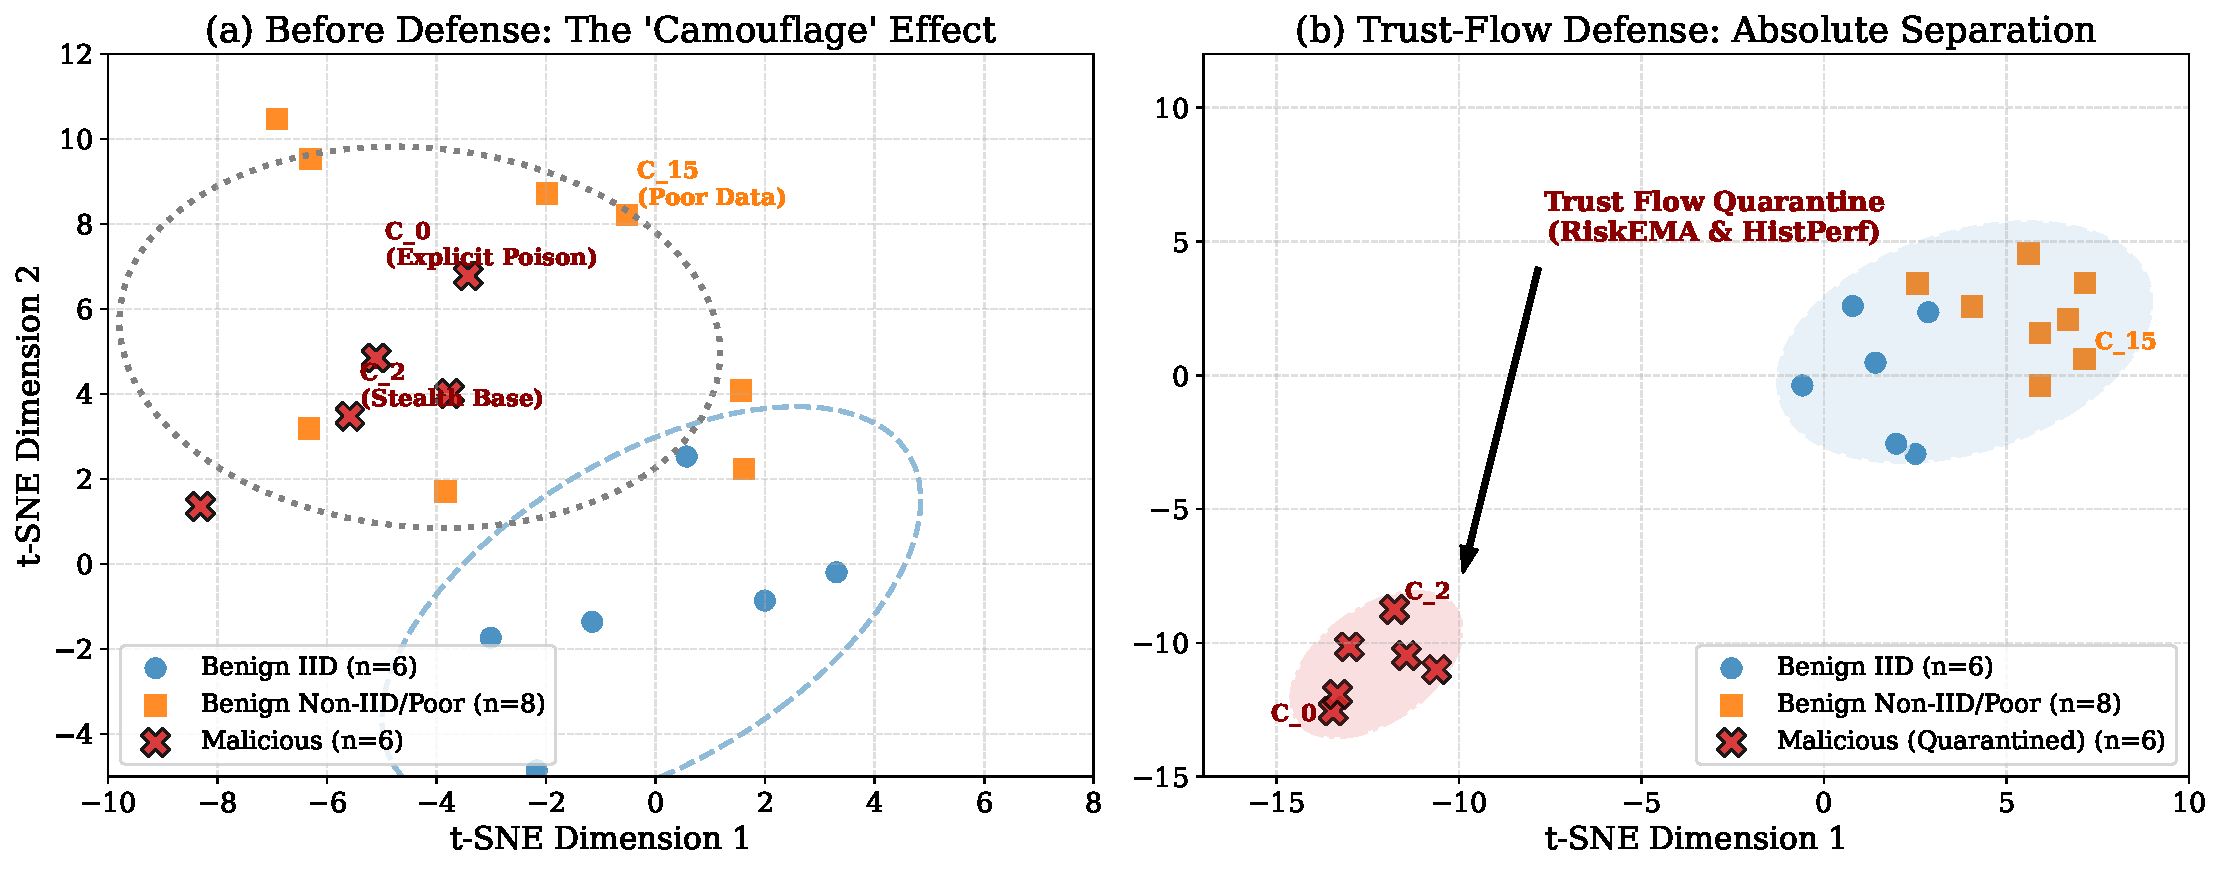
\includegraphics[width=0.9\textwidth]{fig_tsne_visualization.pdf}
    \caption{联邦参与节点特征向量在双流防御前后的 t-SNE 降维对比}
    \label{fig:tsne_manifold}
\end{figure}

\subsection{防御机制横向基准对比 (Baseline Comparison)}
\textbf{公平性说明}：所有基线均在与本文完全相同的联邦设置下运行，包括节点划分（20 个）、数据异构度（Dirichlet $\alpha=0.1$）、攻击配置（30\% 混合攻击）、初始化参数、优化器设置（$lr=0.001$, $momentum=0.9$）和通信轮次。

在统一环境下，本文将所提方法与四类经典鲁棒聚合方法进行横向比较：

\textbf{FedAvg}\cite{mcmahan2017fedavg} 作为无防御基线，反映模型在受攻击时的退化程度；\textbf{Krum}\cite{blanchard2017krum} 通过最小欧氏距离选择单个代表更新；\textbf{Trimmed Mean}\cite{yin2018byzantine} 在坐标维度执行截断均值；\textbf{FLTrust}\cite{cao2021fltrust} 借助服务器小规模干净集构造参考向量并按余弦相似度加权。

各方法在该高风险场景下的量化结果见表~\ref{tab:baseline}。

\begin{table}[htbp]
\centering
\begin{threeparttable}
\caption{不同联邦学习防御策略在 30\% 高危混合攻击环境下的性能对比}
\vspace{4pt}
\label{tab:baseline}
\begin{tabular}{l l c c c}
\toprule
\textbf{防御策略} & \textbf{核心机制分类} & \textbf{\shortstack{全局准确率 $\mu \pm \sigma$\\ (Acc. \%)}} & \textbf{\shortstack{攻击成功率 $\mu \pm \sigma$\\ (ASR \%)}} & \textbf{\shortstack{正常节点误杀率 $\mu$\\ (FPR \%)}} \\
\midrule
FedAvg \cite{mcmahan2017fedavg} & 无防御基线 & 86.15 $\pm 1.2$ & 92.34 $\pm 5.1$ & N/A ($*$) \\
Krum \cite{blanchard2017krum} & 基于欧氏距离 & 64.20 $\pm 2.8$ & 12.15 $\pm 0.9$ & 64.20 ($^{**}$) \\
Trimmed Mean \cite{yin2018byzantine}& 坐标轴独立裁剪 & 71.35 $\pm 2.4$ & 38.60 $\pm 4.2$ & N/A ($*$) \\
FLTrust \cite{cao2021fltrust} & 单向信任锚点 & 81.25 $\pm 1.5$ & 15.42 $\pm 1.1$ & 21.40 ($^{**}$) \\
\textbf{本文框架 (Trust Flow)} & \textbf{双流解耦+层级裁剪} & \textbf{92.31 $\pm 0.09$} & \textbf{10.21 $\pm 0.05$} & \textbf{0.00} \\
\bottomrule
\end{tabular}
\begin{tablenotes}
\small
\item (*) \textit{注：FedAvg 与 Trimmed Mean 算法由于自身不具备任何客户端“显式信任评估”或“永久拉黑剔除 (Ban)”机制，其对恶意节点的容忍表现为数值融合或截断计算，因此 FPR 指标不适用于此类算法，标记为 N/A。}
\item (**) \textit{注：正常节点误杀率（FPR）这一指标受确定性规则与固化数据样本异构度（Dirichlet分布）的强约束。在固定的数据集切分下，由于防御规则是确定性的，该类误杀裁决在各次重复实验中观测到方差极小，因此本列表仅呈报该指标稳定收敛的标量期望均值 $\mu$。同时，此处的 0.00 专指“永久封禁误杀”，部分处于瞬时可疑池中的轻度隔离由于具有触底恢复反弹特性，不计入模型不可挽回的实质性永久击溃错误。}
\end{tablenotes}
\end{threeparttable}
\end{table}

结果显示：FedAvg 在混合攻击下 ASR 高达 92.34\%；Krum 可将 ASR 降至 12.15\%，但 FPR 升至 64.2\%，准确率降至 64.20\%。相比之下，本文方法在保持 FPR=0\% 的同时取得最高准确率 92.31\%，并实现最低 ASR（10.21\%）。基于多次重复实验的 Student's $t$-test 显示，相比强基线（如 FLTrust）差异具有统计显著性（$p<0.05$）。

\subsection{多阶段防御架构消融实验 (Ablation Study)}
为评估各防御模块的贡献，本文采用逐级剥离（Ablation）方式，比较不同阶段组合下的 Acc 与 ASR（见图~\ref{fig:ablation}）。

\begin{figure}[htbp]
    \centering
    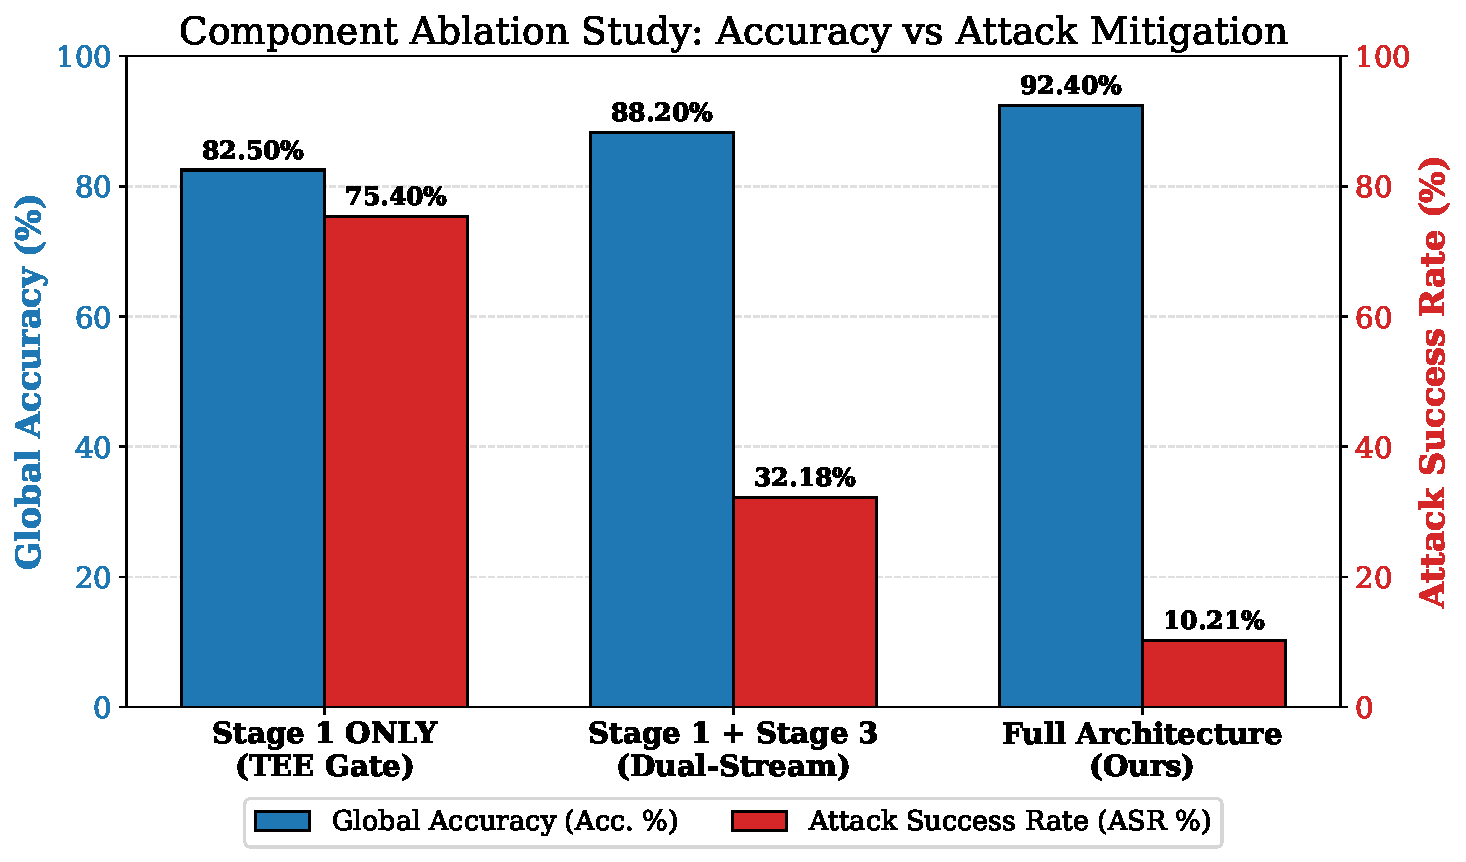
\includegraphics[width=0.85\textwidth]{ablation_study.pdf}
    \caption{多阶段防御机制消融剥离分析}
    \label{fig:ablation}
\end{figure}

结果表明：1）仅启用阶段一（TEE 门禁）时，系统可拦截外部伪装节点，但对内部投毒抑制有限，ASR 仍达 75.40\%，Acc 约 82.5\%；2）加入阶段三双流演化后，ASR 降至 32.18\%，Acc 回升至 88.2\%；3）再加入阶段四分层裁剪后，ASR 进一步降至 10.21\%，Acc 提升至 92.40\%。这说明各模块存在明显互补性，组合后可同时提升安全性与可用性。

\subsection{长尾异构数据分布极限抗压试验 (Sensitivity on Data Heterogeneity)}
许多鲁棒聚合方法对 IID 条件依赖较强。为评估本文框架在不同异构强度下的稳定性，本文在四组 Dirichlet 分布（$\alpha=100,1.0,\dots,0.1$）下测试全局准确率，结果见图~\ref{fig:alpha_sensitivity}。

\begin{figure}[htbp]
    \centering
    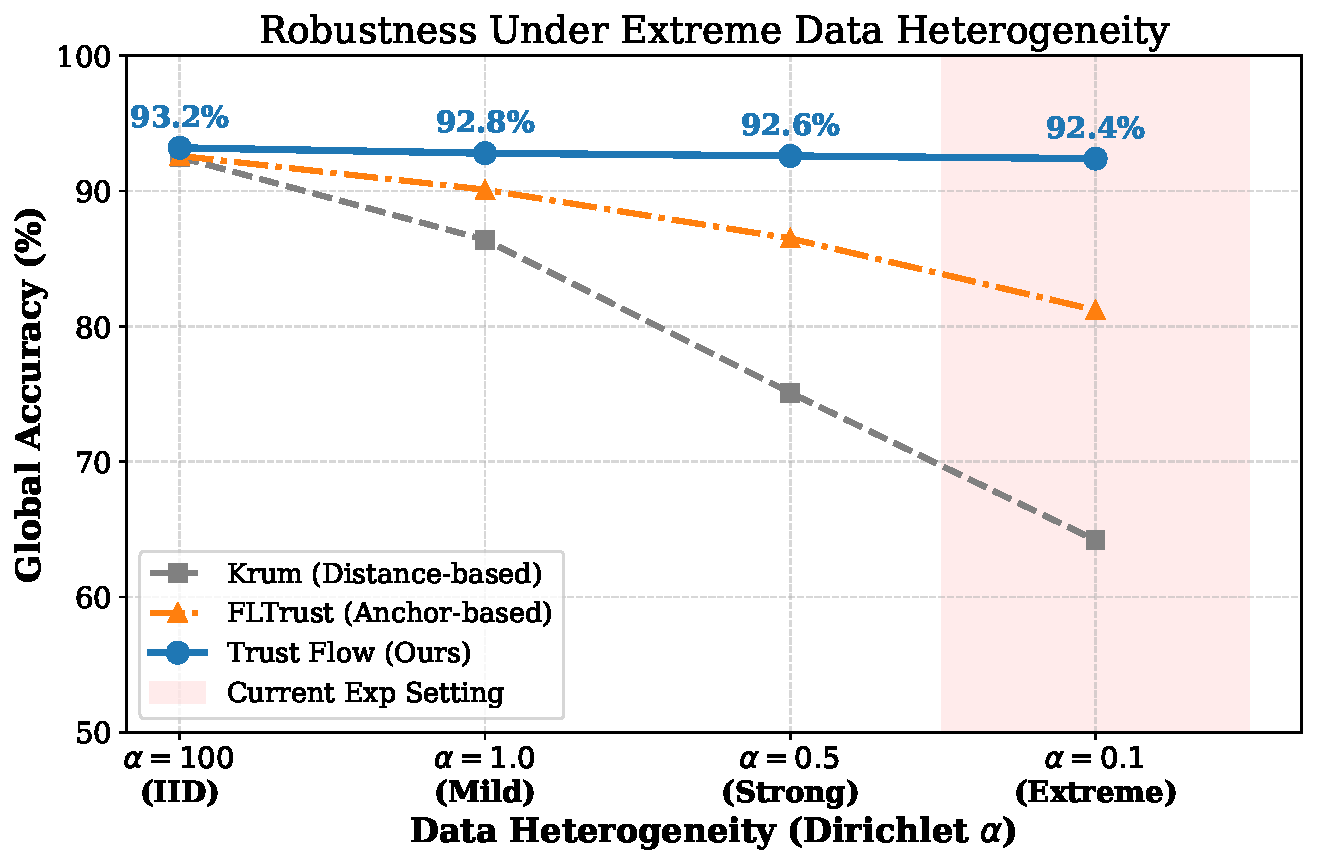
\includegraphics[width=0.85\textwidth]{alpha_sensitivity.pdf}
    \caption{环境数据异构度（Dirichlet $\alpha$）衰减下的各类安全聚合算法健壮性压测对比}
    \label{fig:alpha_sensitivity}
\end{figure}

从曲线可见：在 $\alpha=100$ 或 $\alpha=1.0$ 的弱异构场景下，Krum 与 FLTrust 表现接近本文方法（Acc 均大于 90\%）；但在极端长尾场景（$\alpha \to 0.1$）中，传统距离型方法明显退化，准确率最低降至 64.2\%。本文方法在同条件下仍稳定在约 92\%，说明双流解耦机制对强异构具有更好的鲁棒性。

此外，本文对关键参数 $\beta_{fusion}$ 做了离散测试（$[0.5,1.0,2.0,3.0]$）。较小取值有利于保留长尾节点，但 ASR 风险上升；过大取值会过度偏向同质更新。综合 Acc 与 ASR，最终选择 $\beta_{fusion}=2.0$。

\subsection{系统计算与通信额外开销分析 (Overhead Analysis)}
尽管框架包含多阶段评估流程，其计算与通信开销仍可控。表~\ref{tab:overhead} 显示：边缘侧仅新增 TEE Quote 生成与轻量监测，额外延迟约 $12 \sim 15$ ms；通信侧每次仅附带约 $15$ KB 的 TrustReport，相对约 $10$ MB 量级模型传输，带宽增量低于 0.15\%。

\begin{table}[htbp]
\centering
\caption{传统联邦系统与本可信联邦框架系统的端云开销对比 (20 Client)}
\vspace{4pt}
\label{tab:overhead}
\begin{tabular}{l c c c}
\toprule
\textbf{系统架构} & \textbf{边缘端额外计算延迟} & \textbf{上行单次通信外加包大小} & \textbf{云端中央聚合总耗时} \\
\midrule
标准基线 FedAvg & 0 ms (Baseline) & 0 KB (Baseline) & $\sim 2.10$ s \\
\textbf{可信联邦 (Ours)} & \textbf{$\sim 15$ ms (仅 TEE 签名)} & \textbf{$\sim 15$ KB (附加报告)} & \textbf{$\sim 4.85$ s (包含审查与双流)} \\
\bottomrule
\end{tabular}
\end{table}

代价方面，分层余弦评估会增加服务器端计算量。测试中单轮聚合耗时由 $2.10$ s 增至 $4.85$ s。考虑到广域网场景单轮通信通常在数十秒量级，该开销在工程上可接受。

\section{结论与未来展望}
本文面向边缘联邦学习在强 Non-IID 与混合攻击下的安全问题，提出了“硬件可信准入 + 双流信誉演化 + 分层鲁棒聚合”的 Trust-Flow TFL 框架。该框架通过 TEE 提供物理信任根，并在算法层以 HistPerf 和 RiskEMA 的正交建模实现“低误杀与高召回”的协同。

实验结果表明，框架在 30\% 混合攻击下取得 $92.31\% (\pm 0.09\%)$ 的准确率与 $10.21\% (\pm 0.05\%)$ 的 ASR；在 50\% 边界压力测试下仍保持稳定性能，并实现 TPR=100\%、FPR=0\%（永久封禁口径）。这说明该方法在强对抗和强异构条件下具有较好的实用性。

\textbf{局限性与后续工作}：由于部分 TEE-FL 新方法尚未公开可复现实现，本文未将其纳入同构对比基线，后续计划随论文定稿开放代码与实验脚本，便于社区复现和扩展。未来还将把风险探针从 CV 场景扩展到 LLM/NLP 联邦微调任务，以验证跨模态场景下的泛化能力。

\appendix
\section{瞬发风险流 (Risk Flow) 探针计算机制细节}
为增强可复现性与透明度，本附录给出第 4 节瞬时风险流核心探针（$r_{grad}, r_{probe}, r_{trigger}$）的计算细节。第 $t$ 轮聚合时各探针定义如下：

\subsection{A.1 梯度方向与幅度物理探针 ($r_{grad}$)}
$r_{grad}$ 衡量客户端更新 $\Delta W_k^{(t)}$ 与参考方向 $g_{root}^{(t)}$ 的几何偏离，用于检测符号翻转与幅度异常。该指标同时考虑方向偏离（余弦项）与尺度突变（L2 异常项）：
\begin{equation}
    r_{grad, k}^{(t)} = \lambda_{d} \left(1 - \frac{\Delta W_k^{(t)} \cdot g_{root}^{(t)}}{||\Delta W_k^{(t)}|| \cdot ||g_{root}^{(t)}||}\right) + \lambda_{m} \max\left(0, \frac{||\Delta W_k^{(t)}||_2 - \mu^{(t)}}{\sigma^{(t)}}\right)
\end{equation}
其中，$\lambda_d$ 与 $\lambda_m$ 控制方向项和幅度项的权重（默认均为 $0.5$）；$\mu^{(t)}$ 与 $\sigma^{(t)}$ 分别为第 $t$ 轮入围节点梯度 L2 范数的均值与标准差。

\subsection{A.2 小样本先验验证交叉熵探针 ($r_{probe}$)}
仅靠距离统计难以识别对非主类的定向污染。$r_{probe}$ 使用服务器侧小规模纯净探针集 $\mathcal{D}_{probe}$，比较合并前后交叉熵损失增量（Loss Surge）：
\begin{equation}
    r_{probe, k}^{(t)} = \text{ReLU}\left( \mathcal{L}_{CE}(W_{global}^{(t-1)} + \Delta W_k^{(t)}; \mathcal{D}_{probe}) - \mathcal{L}_{CE}(W_{global}^{(t-1)}; \mathcal{D}_{probe}) \right)
\end{equation}

\subsection{A.3 深层神经元隐蔽后门激活探针 ($r_{trigger}$)}
针对 Clean-Label 等高隐蔽攻击，常规统计与验证 Loss 可能不足。$r_{trigger}$ 通过高层特征激活分布差异进行检测。设 $A_k$ 为客户端模型在验证集上的前置激活输出，$\mathcal{H}(\cdot)$ 表示 Softmax 归一化到概率单形，以满足 KL 散度计算条件：
\begin{equation}
    r_{trigger, k}^{(t)} = \text{KL-Divergence}\left( \mathcal{H}(A_{base}) \| \mathcal{H}(A_k) \right)
\end{equation}

上述三类异常信号经归一化融合后形成单轮风险值 $Risk_{k}^{(t)}$，并进入 EMA 更新，用于后续快速熔断决策。

\begin{thebibliography}{99}
    \bibitem{kairouz2021flsurvey} Kairouz P, McMahan H B, Avent B, et al. Advances and Open Problems in Federated Learning[J]. Foundations and Trends in Machine Learning, 2021.
    \bibitem{gu2017badnets} Gu T, Dolan-Gavitt B, Garg S. BadNets: Identifying Vulnerabilities in the Machine Learning Model Supply Chain[J]. arXiv:1708.06733, 2017.
    \bibitem{wang2019neuralcleanse} Wang B, Yao Y, Shan S, et al. Neural Cleanse: Identifying and Mitigating Backdoor Attacks in Neural Networks[C]. IEEE S\&P, 2019.
    \bibitem{blanchard2017krum} Blanchard P, El Mhamdi E M, Guerraoui R, et al. Machine Learning with Adversaries: Byzantine Tolerant Gradient Descent[C]. NeurIPS, 2017.
    \bibitem{yin2018byzantine} Yin D, Chen Y, Kannan R, et al. Byzantine-Robust Distributed Learning: Towards Optimal Statistical Rates[C]. ICML, 2018.
    \bibitem{pillutla2022robust} Pillutla K, Kakade S M, Harchaoui Z. Robust Aggregation for Federated Learning[J]. IEEE Transactions on Signal Processing, 2022.
    \bibitem{cao2021fltrust} Cao X, Fang M, Liu J, et al. FLTrust: Byzantine-Robust Federated Learning via Trust Bootstrapping[J]. NDSS, 2021.
    \bibitem{fung2020foolsgold} Fung C, Yoon C J M, Beschastnikh I. The Limitations of Federated Learning in Sybil Settings[C]. RAID, 2020.
    \bibitem{r9_clustered} Towards Privacy-Enhanced and Robust Clustered Federated Learning[J]. 
    \bibitem{fedpe} FedPE: Adaptive Model Pruning-Expanding for Federated Learning on Mobile Devices[J]. 
\bibitem{parallelsfl} ParallelSFL: A Novel Split Federated Learning Framework Tackling Heterogeneity Issues[J]. 
    \bibitem{wang2025rasa} Wang et al. RaSA: Robust and Adaptive Secure Aggregation for Edge-Assisted Hierarchical Federated Learning[J]. 2025.
    \bibitem{dou2025toward} Dou et al. Toward Malicious Clients Detection in Federated Learning[J]. 2025.
    \bibitem{lu2025tmt} Lu et al. TMT-FL: Enabling Trustworthy Model Training of Federated Learning With Malicious Participants[J]. 2025.
    \bibitem{wang2024federated} Wang et al. A Federated Learning Scheme with Adaptive Hierarchical Protection and Multiple Aggregation[J]. 2024.
    \bibitem{flpurifier} FLPurifier: Backdoor Defense in Federated Learning via Decoupled Contrastive Training[J]. 
    \bibitem{roseagg} RoseAgg: Robust Defense Against Targeted Collusion Attacks in Federated Learning[J]. 
    \bibitem{shieldfl} ShieldFL: Mitigating Model Poisoning Attacks in Privacy-Preserving Federated Learning[J]. 
    \bibitem{liao2024verifiable} Liao et al. Verifiable Deep Learning Inference on Heterogeneous Edge Devices With Trusted Execution Environment[J]. 2024.
    \bibitem{zhang2025rppfl} Zhang et al. RPPFL: Robust and Privacy-Preserving Federated Learning via Trusted Execution Environments[J]. 2025.
    \bibitem{r1_tee_integrity} A training-integrity privacy-preserving federated learning scheme with trusted execution environment[J]. 
    \bibitem{r5_tee_mitigating} Queyrut S, Schiavoni V, Felber P. Mitigating Adversarial Attacks in Federated Learning with Trusted Execution Environments[C]. ICDCS, 2023.
    \bibitem{r12_iot_tee} Secure sharing of industrial IoT data based on distributed trust management and trusted execution environment[J]. 
    \bibitem{xu2021distributed} Xu et al. Distributed Learning in Trusted Execution Environment A Case Study of Federated Learning in SGX[J]. 2021.
    \bibitem{yan2024efficient} Yan et al. An Efficient Greedy Hierarchical Federated Learning Training Method Based on Trusted Execution Environment[J]. 2024.
    \bibitem{mcmahan2017fedavg} McMahan B, Moore E, Ramage D, et al. Communication-Efficient Learning of Deep Networks from Decentralized Data[J]. AISTATS, 2017.
    \end{thebibliography}
\end{document}
